\documentclass[11pt]{article}
\renewcommand{\baselinestretch}{1.05}
\usepackage[spanish]{babel}
\usepackage[utf8]{inputenc}
\usepackage{lipsum}

\usepackage{amsmath,amsthm,verbatim,amssymb,amsfonts,amscd}
\usepackage{graphicx, wrapfig}
\usepackage{float}
\usepackage{caption, subcaption}
\usepackage{tkz-fct}
\usetikzlibrary{babel}
\usepackage{pgfplots}
\usepackage{enumitem}
\usepackage{multicol, vwcol}
\usepackage{listingsutf8}
\usepackage{color}
\usepackage{hyperref}
\usepackage{booktabs}


\usepackage[sorting=none]{biblatex}
\bibliography{bibliography.bib}

\hypersetup{
    bookmarks=true,         % show bookmarks bar?
    unicode=false,          % non-Latin characters in Acrobat’s bookmarks
    pdftoolbar=true,        % show Acrobat’s toolbar?
    pdfmenubar=true,        % show Acrobat’s menu?
    pdffitwindow=false,     % window fit to page when opened
    pdfstartview={FitH},    % fits the width of the page to the window
    pdftitle={Visión por computador - Trabajo final},    % title
    pdfauthor={Francisco Luque, Maria del Mar Ruiz},     % author
    pdfsubject={Visión por computador},   % subject of the document
    pdfnewwindow=true,      % links in new PDF window
    colorlinks=true,        % false: boxed links; true: colored links
    linkcolor=black,          % color of internal links (change box color with linkbordercolor)
    citecolor=cyan,         % color of links to bibliography
    filecolor=magenta,      % color of file links
    urlcolor=blue           % color of external links
}

\setlength{\parindent}{0pt}
\topmargin0.0cm
\headheight0.0cm
\headsep0.0cm
\oddsidemargin0.0cm
\textheight23.0cm
\textwidth16.5cm
\footskip1.0cm
\theoremstyle{plain}

\newtheorem{theorem}{Teorema}
\newtheorem{corollary}{Corolario}
\newtheorem{lemma}{Lema}
\newtheorem{proposition}{Proposición}
\theoremstyle{definition}
\newtheorem{definition}{Definición}
\newtheorem{example}{Ejemplo}

\newcommand{\N}{\mathbb{N}}
\newcommand{\Z}{\mathbb{Z}}
\newcommand{\Q}{\mathbb{Q}}
\newcommand{\C}{\mathbb{C}}
\newcommand{\R}{\mathbb{R}}

\begin{document}

\begin{titlepage}
  \centering
  {\scshape\LARGE Universidad de Granada \par}
  \vspace{1cm}
  {\scshape\Large Visión por computación \par}
  \vspace{1.5cm}
  {\huge\bfseries Clasificación de imágenes usando CNNs \par}
  \vspace{2cm}
  {\Large\itshape Francisco Luque Sánchez \\
    María del Mar Ruiz Martín\par}
  \vspace{2cm}
  
\includegraphics[width=.3\textwidth]{logougr.png}\par\vspace{1cm}
  % Bottom of the page
  {\large \today\par}
\end{titlepage}

\newpage

\tableofcontents

\newpage

\section{Introducción}

En esta práctica se tratará el problema de la clasificación de objetos
en imágenes, utilizando concretamente redes neuronales convolucionales
(\textit{CNNs}). El problema que se abordará consiste en tratar de
distinguir perros de gatos utilizando estos modelos. Se comenzará con
un modelo simple, el cual se irá modificando para tratar de mejorar su
capacidad para clasificar.

\subsection{Conjunto de datos utilizado}

El conjunto de datos utilizado se ha generado utilizando las bases de
datos mostradas en \cite{db1, db2, db3}. Se han extraído todas las
imágenes de las mismas y etiquetado en dos clases (perros y gatos),
obteniéndose un conjunto total de unos 13000 gatos y 25000
perros. Dicho conjunto se ha dividido en dos subconjuntos, un conjunto
de entrenamiento (unos 25500 ejemplos) y uno de test (en torno a 12500
ejemplos), tratando de mantener la proporción de perros y gatos lo más
parecida posible en ambos conjuntos.\\

En cuanto al tamaño de las imágenes utilizado, se han redimensionado
todas ellas a un tamaño de $64 \times 64$ píxeles con codificación RGB
(es decir, se trabajará con imágenes de entrada de tamaño
$(64, 64, 3)$. Se utilizan imágenes de tan pequeño tamaño porque el
uso de imágenes de mayor tamaño provoca un aumento de tamaño muy
notable de la red neuronal utilizada, lo que se traduce en un aumento
del tiempo de cómputo muy considerable. Además, se comenzó haciendo
una prueba con imágenes de tamaño $128 \times 128$, y la diferencia en
los resultados obtenidos no era significativa. Finalmente, este
trabajo tiene la finalidad de estudiar las diferencias de capacidad de
clasificación de las redes neuronales convolucionales en función a su
estructura y parámetros, por lo que en principio no necesitamos crear
ejemplos muy potentes que permitan una clasificación muy precisa.
Se decide por tanto utilizar imágenes de este tamaño, aunque pueda
provocar que en fases finales del trabajo se pierda un poco de capacidad
de predicción al no utilizar imágenes de tamaño mayor.

\subsection{Aspectos de implementación}

Todo el código se ha desarrollado utilizando el \textit{framework}
TensorFlow \cite{tf}, que es una librería de código abierto
desarrollada por Google, orientada a la implementación de soluciones
utilizando inteligencia artificial. Esta librería permite la definición
de forma sencilla de estructuras de redes neuronales de varios tipos,
entre ellas redes neuronales convolucionales, que es el tipo de redes
en las que se centra el trabajo. Además, permite especificar los recursos
del equipo que se destinan a cómputo, dando gran flexibilidad al programador
a la hora de hacer los experimentos. El primer modelo desarrollado, en
particular, se ha hecho utilizando un tutorial de la documentación
del \textit{framework}, que se puede consultar en \cite{cnn-tutorial}.\\

El código se ha estructurado en 5 archivos distintos para cada modelo.
En el archivo \texttt{model.py} se establece la estructura de la red
neuronal. En los archivos \texttt{model\_train.py} y
\texttt{model\_test.py} se establece la ejecución de las operaciones
de entrenamiento y test.  En el archivo \texttt{input.py} se
implementan las funciones de lectura de imágenes desde
archivo. Finalmente, el archivo \texttt{predict\_image.py} permite que
se pase un nombre de imagen como argumento, y se utiliza el modelo
entrenado para predecir si en dicha imagen hay un perro o un gato.

\section{Modelos implementados}

\subsection{Model básico (\texttt{base\_model})}

Comenzamos describiendo el primer modelo implementado. Es el modelo
más simple de los estudiados. Pasamos a ver su estructura.

\subsubsection{Estructura de la red}

La primera de las redes se organiza de la siguiente manera. Recibe un
batch de 128 imágenes de tamaño $64 \times 64\times 3$. La primera
operación que realiza consiste en una capa de convolución que extrae
64 filtros para cada una de las imágenes. Después, tiene una capa de
pool que reduce el tamaño de las imágenes a la mitad, por lo que tras
esta capa se tiene un conjunto de imágenes de tamaño
$128 \times 32 \times 32 \times 64$. Tras esto, se redimensiona la
capa para que tenga una forma de $128 \times 65536$ características, y
se pasa dicho vector a una capa completamente conectada de tamaño
$65536 \times 348$.  Esta capa completamente conectada se conecta a
otra capa completamente conectada con dos neuronas, que nos darán la
probabilidad de que el elemento pertenezca a la clase gato (neurona 0)
o la clase perro (neurona 1). Las funciones de activación de todas las
capas es la función \textit{Relu}. El esquema de la misma es el siguiente:

\begin{figure}[H]
  \centering
  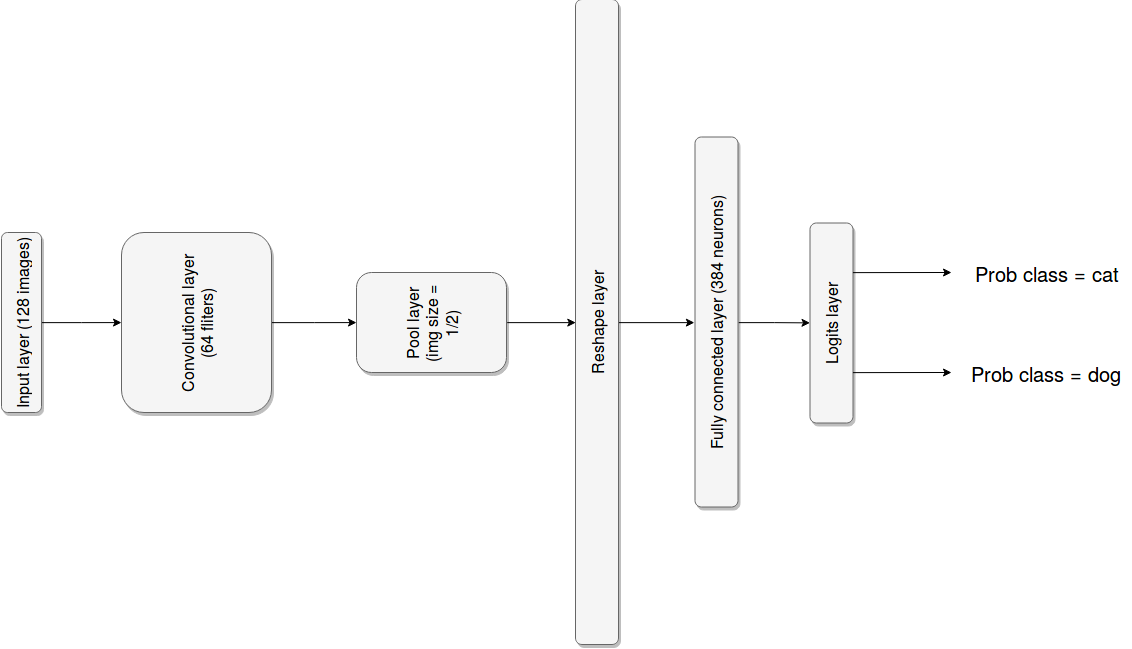
\includegraphics[width=.7\textwidth]{imgs/simple_model.png}  
  \caption{Esquema del modelo simple de red neuronal convolucional}
\end{figure}

\subsubsection{Aprendizaje de la red}

Una vez definida la estructura de la red, vamos a explicar ligeramente
el funcionamiento del aprendizaje de la misma. En cada etapa del
aprendizaje, se genera aleatoriamente del conjunto de imágenes de
entrenamiento un subconjunto de 128 ejemplos. La red neuronal
clasifica dichas imágenes, otorgando una probabilidad a cada una de
ellas de que pertenezca a una clase o a la otra.  Una vez hecha la
clasificación, se calcula el error cometido como la media de los
errores cometidos. El error cometido es la diferencia entre la
probabilidad estimada para cada clase y la clase real de la imagen.
Una vez calculado dicho error, se propaga con un gradiente descendente
para modificar los pesos de todas las capas. La tasa de aprendizaje es
constante durante todo el entrenamiento, con un valor de $0.001$.
Se realizan 8000 pasos de aprendizaje.

\subsubsection{Evaluación del aprendizaje durante el entrenamiento}

Para ir viendo cómo evoluciona el aprendizaje de la red durante el
entrenamiento, se ejecuta simultáneamente un test sobre la red
neuronal. Este test coge un conjunto aleatorio de 10000 imágenes
del conjunto de test y lo clasifica utilizando la red neuronal.
Una vez clasificadas las mismas (se obtiene la probabilidad de que
cada una de las imágenes pertenezca a una de las dos clases, y se
devuelve como clase la que tenga una probabilidad mayor), se hace
el cociente entre el total de ejemplos bien clasificados y el número
de ejemplos totales, obteniéndose así el tanto por uno de instancias
bien clasificadas.

\subsubsection{Gráficas de resumen del aprendizaje}

Utilizando una de las utilidades de \textit{TensorFlow}, llamada
\textit{TensorBoard}, se han creado varios gráficos que permiten ver
cómo evoluciona la capacidad de predicción de la red en función al
número
de iteraciones de aprendizaje que ha realizado la misma.\\

Nos centraremos principalmente en dos gráficas. Una que muestra la
evolución de la función de pérdida, la cual tratamos de minimizar, y
otra que muestra la capacidad de predicción sobre el conjunto de test.\\

Estas dos gráficas van a ser nuestra principal forma de obtener
información sobre la evolución del aprendizaje de la red neuronal. Una
de las ventajas que ofrece TensorFlow es que permite al programador
establecer, de forma muy simplificada (tiene implementado un sistema
de clases para realizar todo el trabajo), qué variables se quieren
supervisar durante el entrenamiento. De esta manera, podemos colocar
supervisores que mantengan un historial de los pesos de las distintas
capas de la red, de si ciertas neuronas se activan o se inhiben para
una determinada foto, cómo se propagan los gradientes por la red
neuronal con el algoritmo de \textit{backpropagation}... y mostrar
toda esta información a posteriori con una interfaz web (es esta
interfaz la que se conoce como \textit{TensorBoard}). No obstante, en
este trabajo no se mostrará la capacidad completa de esta herramienta,
ya que su configuración es tediosa, y aunque no ralentiza en exceso el
sistema, sí que se puede apreciar cierta pérdida de
rendimiento. Además, la interpretación de estos gráficos, a pesar de
que se muestran de forma bastante clara, no es nada sencilla, y
requieren de un conocimiento previo sobre redes neuronales bastante
profundo. Creemos por tanto que la extracción e interpretación de
dichas gráficas queda fuera de las competencias que intenta cubrir el
trabajo, y por esto mostramos sólo las gráficas cuya interpretación
aporta información realmente relevante sobre el aprendizaje de la
misma.\\

Pasamos entonces a ver la gráfica de la evolución de la función de
pérdida en los distintos pasos de entrenamiento:

\begin{figure}[H]
  \centering 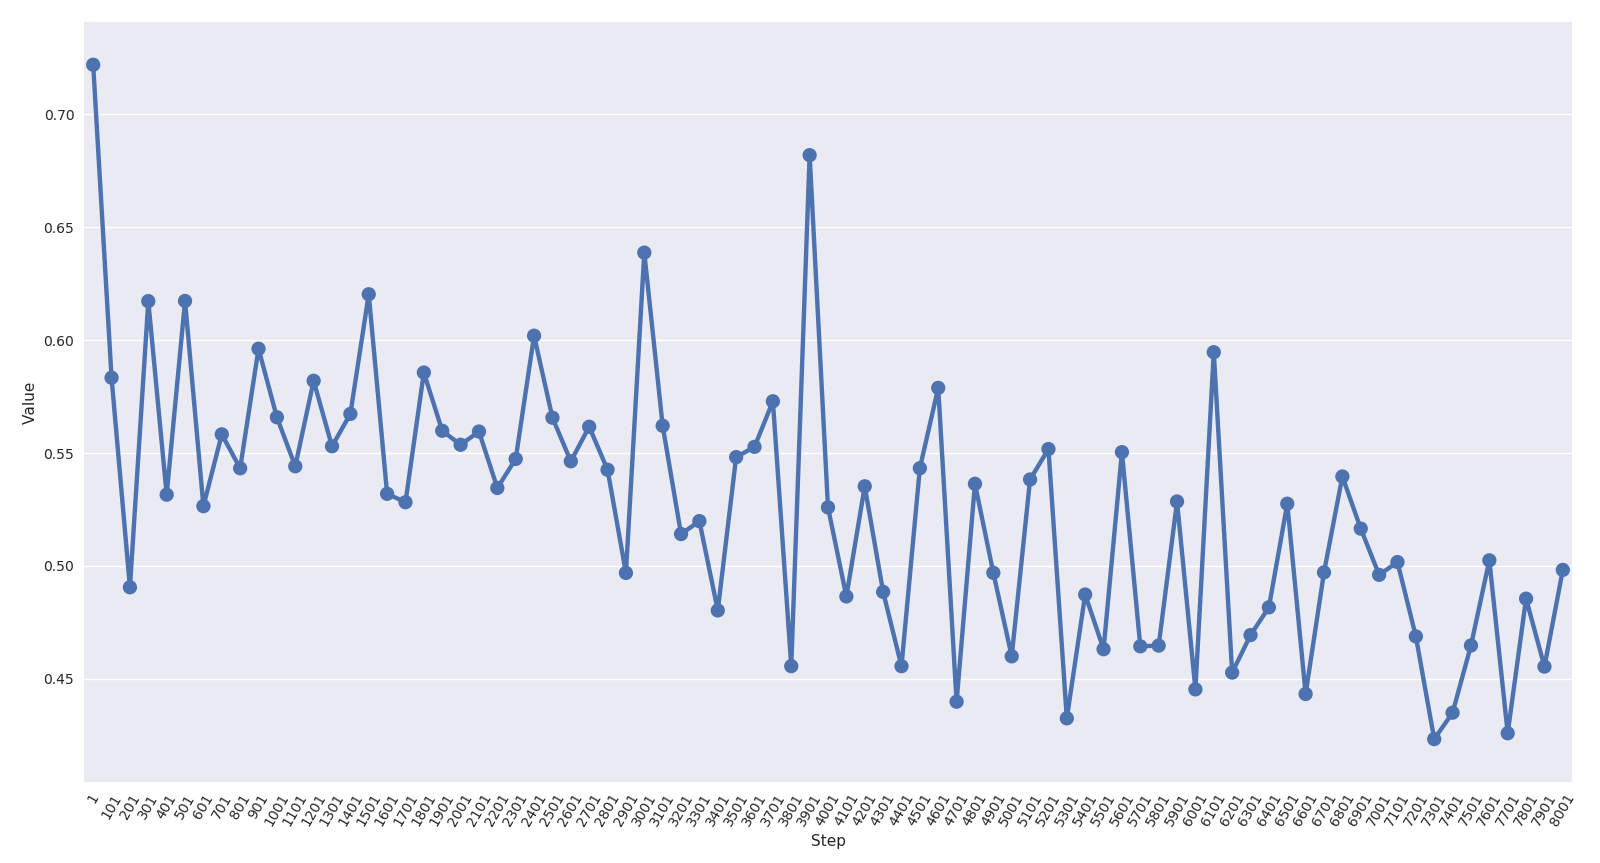
\includegraphics[width=.95\textwidth]{imgs/loss_base}
  \caption{Evolución de la función de pérdida}
\end{figure}

Podemos observar cómo la función de pérdida tiene un comportamiento un
poco caótico en este caso, aunque sí que se observa cierta tendencia
al decrecimiento. Se comienza con un valor cercano a 0.7, el cual se
consigue decrementar hasta 0.43 en la iteración 7700. No obstante, se
ve que el comportamiento no es del todo bueno, ya que se dan muchos
pasos hacia atrás durante el entrenamiento. Pasamos ahora a ver el
comportamiento de la gráfica que muestra la evolución la precisión del
modelo:

\begin{figure}[H]
  \centering 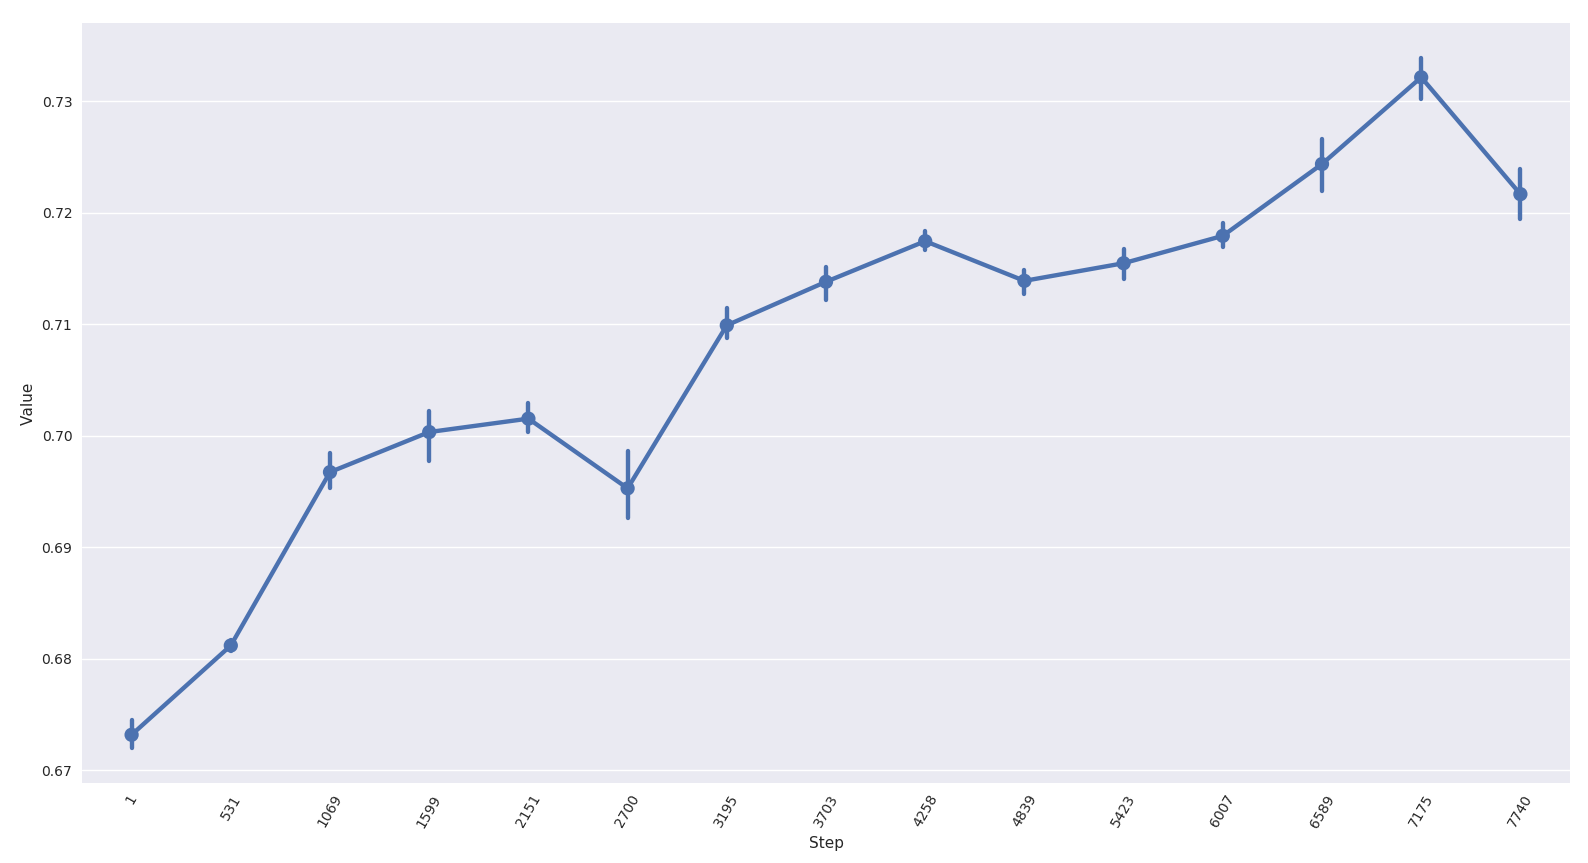
\includegraphics[width=.95\textwidth]{imgs/accuracy_base}
  \caption{Evolución de la precisión de la red neuronal}
\end{figure}

Se puede observar una clara tendencia a la mejora durante todo el
proceso de aprendizaje, aunque no se una mejora muy significativa. El
sistema comienza con una capacidad de predicción de en torno al 67 \%
de efectividad, y consigue mejorar dicha capacidad de predicción hasta
alcanzar una precisión de algo más del 73 \%. No obstante, estos
resultados no son del todo satisfactorios, ya que hemos construido un
modelo muy básico y todavía clasificamos mal algo más de un cuarto de
las instancias que tenemos. En el resto de la práctica se irán
proponiendo mejoras a este modelo básico, que tratarán de mejorar su
capacidad de predicción. La primera de las modificaciones consistirá
simplemente en introducir un \textit{Weight Decay} sobre los pesos de
la red neuronal. Pasamos a describirlo y ver los resultados en la
siguiente sección.

\subsection{Primera modificación: \textit{Weight Decay} (wd\_model)}

Como ya hemos dicho al final de la sección anterior, la primera
modificación que vamos a introducir es lo que se conoce como
\textit{Weight Decay}, o disminución de pesos. Esta modificación
consiste en añadir una penalización a los pesos de la red en la
función de pérdida. Concretamente, se añade un término por cada capa
de la red en las que se aplica, correspondiente a la norma $L_2$ del
vector de pesos, multiplicado por un parámetro a configurar por el
usuario. Esto hace que cada vez que se propaga el error, además de
modificar los pesos en función de la capacidad de predicción, se
reduce la norma del vector, haciendo que los pesos no aumenten
indefinidamente. Veremos que esta modificación nos servirá para que
la red tenga un comportamiento mucho mejor que en el modelo anterior.\\

En cuanto a la estructura de la red y el esquema de aprendizaje de la
misma, no comentaremos nada más, ya que es exactamente la misma que la
que teníamos para el ejemplo anterior. De nuevo tendremos una capa de
convolución, una capa de reducción de tamaño, una de alisamiento de la
dimensión de las imágenes para convertirlas en vectores, una capa
completamente conectada y la salida con dos neuronas. La única
modificación interesante es que los pesos de todas las capas llevan
asociado el \textit{Weight Decay}, lo que se verá claramente en los
valores de la función de pérdida, que tomará valores mucho mayores
(recordemos que en el ejemplo anterior, el valor de la función no
sobrepasaba el valor 1, mientras que ahora comenzará en un valor
cercano a 600). El esquema de aprendizaje es el mismo nuevamente,
utilizándose un esquema de gradiente descendente
con una tasa de aprendizaje constante para propagar el error.\\

Lo que sí tendremos ahora es un aprendizaje mucho más largo.
Mostraremos dos ejecuciones distintas. La primera es una ejecución en
la que se realizan 10000 etapas de aprendizaje. Tras la ejecución, se
observó que, aunque se había mejorado el resultado de la ejecución
básica, la red neuronal no había presentado todavía un estancamiento
en los resultados, por lo que se decide modificar este parámetro, y
establecer el límite de etapas de aprendizaje en 100000. Esta
estimación es muy exagerada, ya que probablemente se produzca antes un
estancamiento, pero como las ejecuciones son costosas, se decide poner
un número desproporcionado de pasos, para cortar el proceso cuando se
observe un estancamiento en la disminución de la función de pérdida.
Más adelante en la práctica se introducirá un método que permita
automatizar el momento del entrenamiento en el que se corta el
aprendizaje. Esto es lo que se llama \textit{Early Stopping}, y
básicamente se basa en hacer que se pare el entrenamiento cuando
se produce un estancamiento en la mejora de la función de pérdida,
esto es, cuando tras un número significativo de iteraciones no se
consigue disminuir el valor de la misma lo suficiente, o no llega
a mejorarse.\\

Pasamos a ver los resultados de las ejecuciones de entrenamiento
conseguidos por esta red neuronal.

\subsubsection{Gráficas de resumen del aprendizaje}

Vamos a ver, como hemos dicho antes, las gráficas de dos ejecuciones
del aprendizaje para este modelo. La primera que se muestra es una
primera ejecución, en la que se establecieron 10000 pasos de
aprendizaje.  Tras ver que al finalizar la ejecución la red neuronal
no se había estancado, se realiza otra ejecución de 100000 pasos para
ver hasta qué punto la red neuronal es capaz de mejorar las
predicciones.  La primera gráfica es la siguiente:

\begin{figure}[H]
  \centering 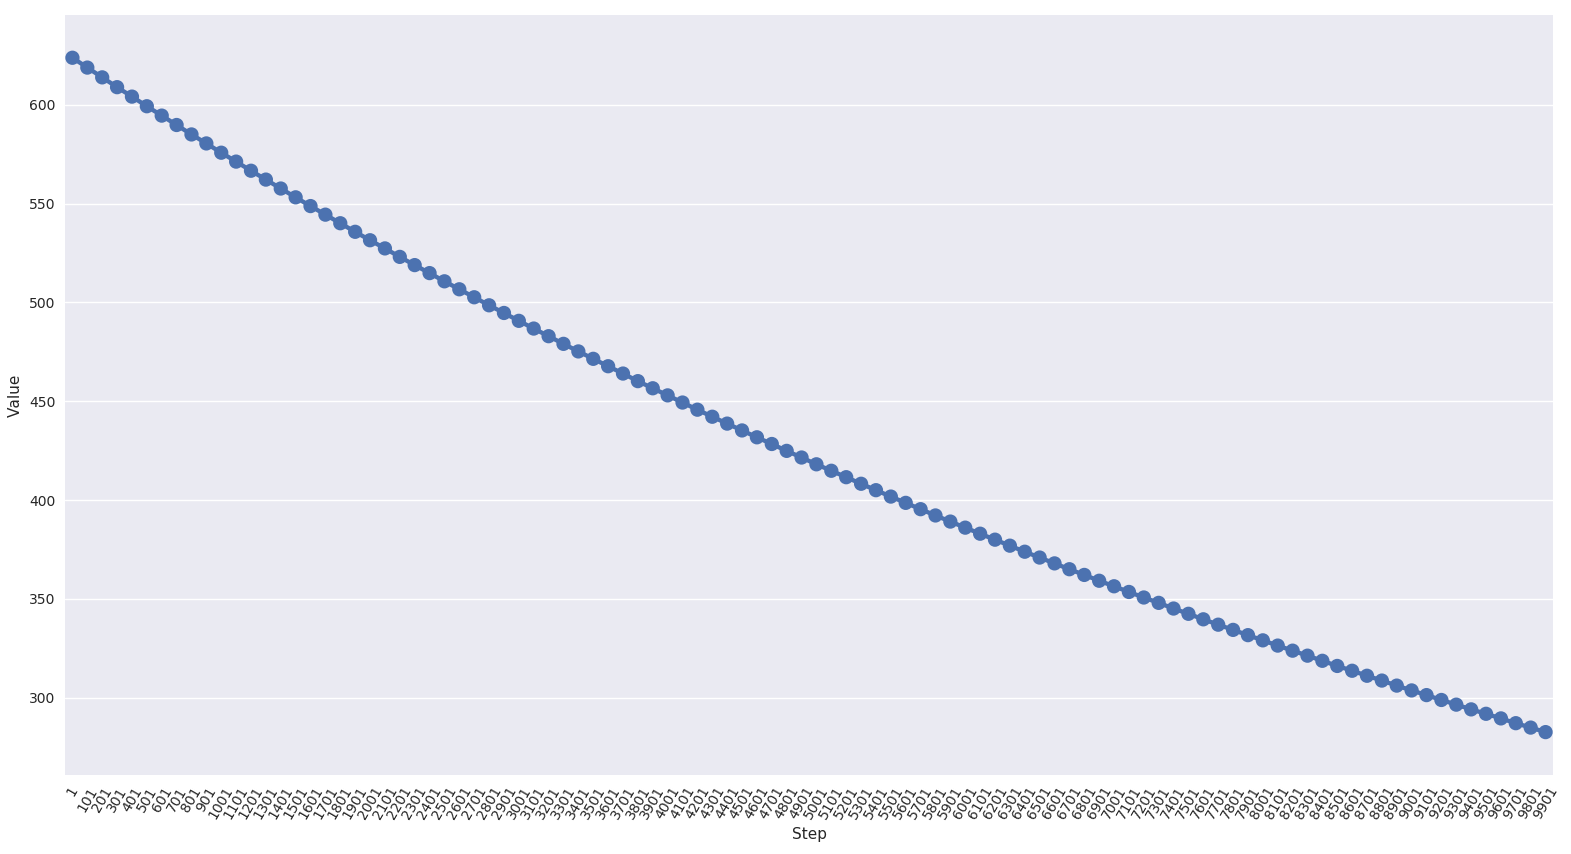
\includegraphics[width=.95\textwidth]{imgs/loss_wd_1}
  \caption{Evolución de la función de pérdida}
\end{figure}

Claramente, la función de pérdida no se ha estabilizado. Si observamos
la gráfica de la capacidad de predicción, tenemos que:

\begin{figure}[H]
  \centering 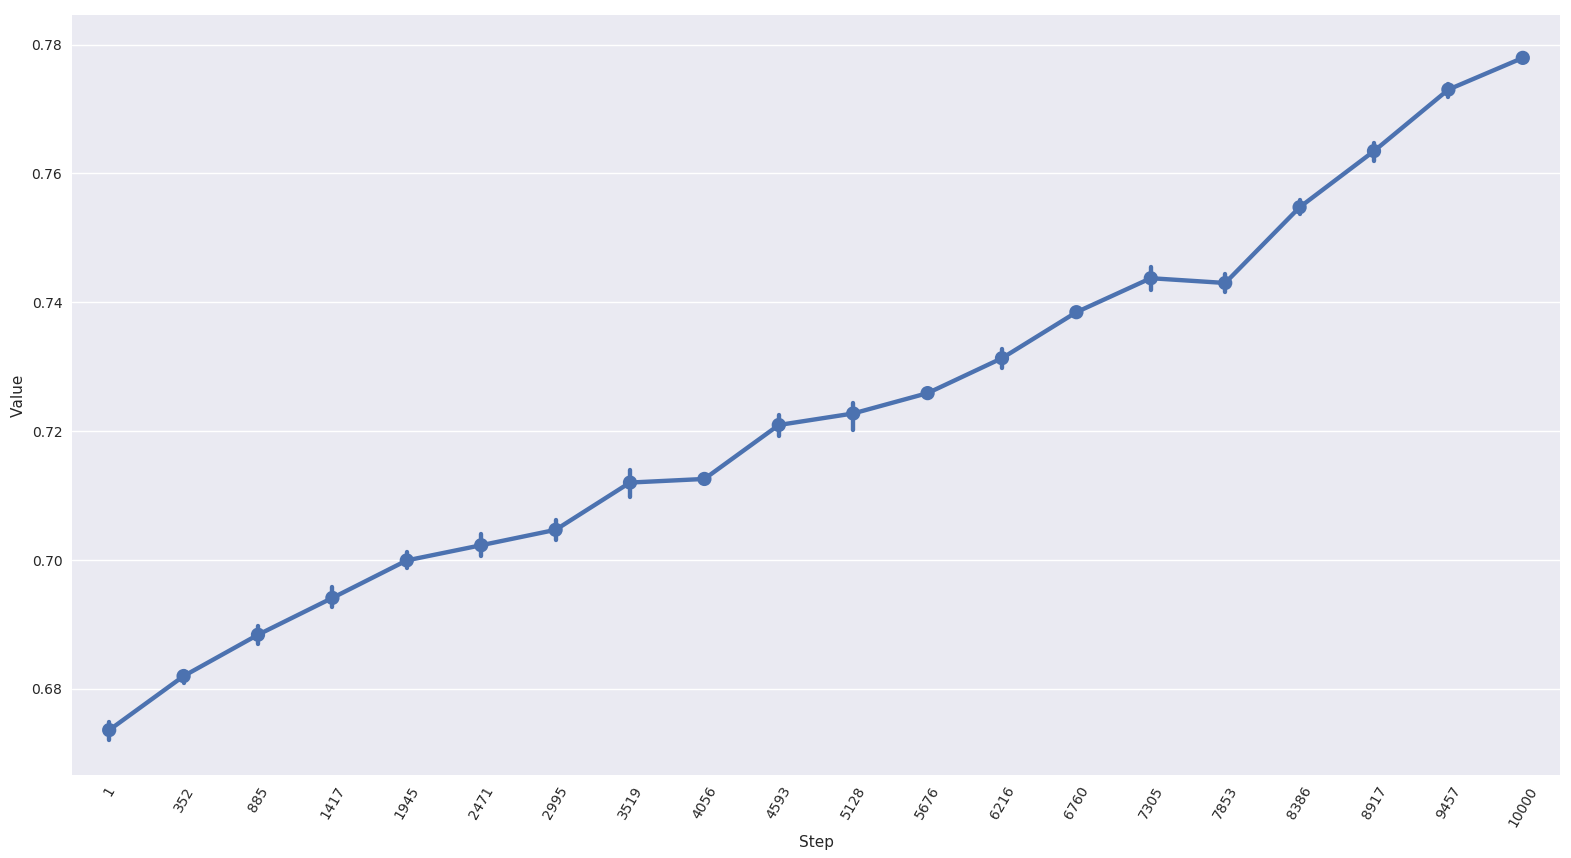
\includegraphics[width=.95\textwidth]{imgs/accuracy_wd_1}
  \caption{Evolución de la capacidad de predicción}
\end{figure}

Donde hemos conseguido un porcentaje de acierto cercano al 78 \%. No
obstante, se ve claramente en ambas gráficas que el resultado es
claramente mejorable. En la segunda ejecución, la gráfica de la
función de pérdida es la siguiente:

\begin{figure}[H]
  \centering 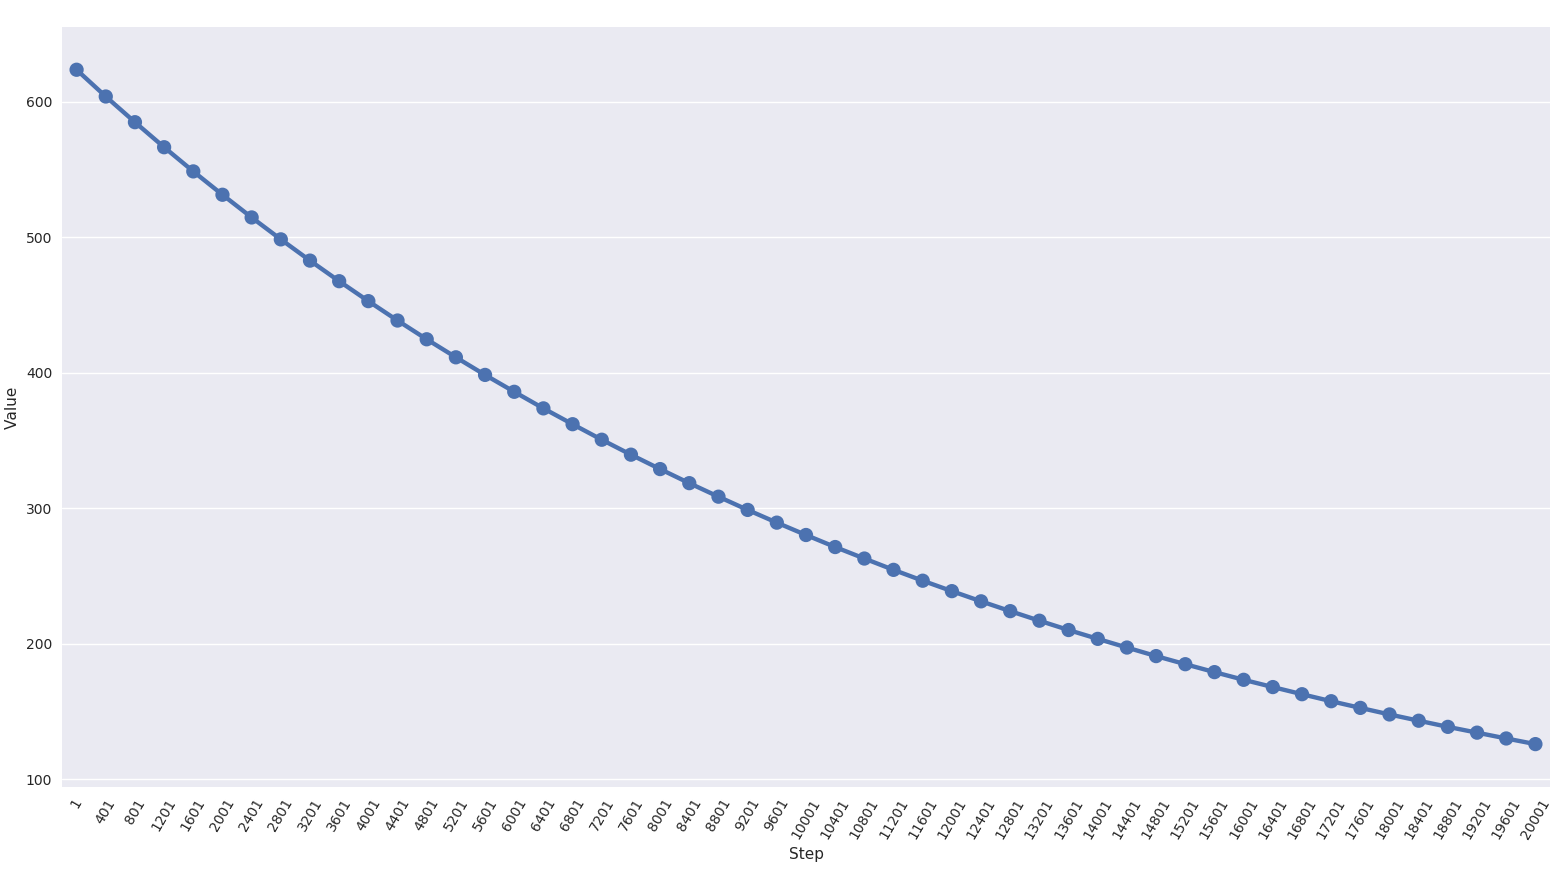
\includegraphics[width=.95\textwidth]{imgs/loss_wd_2}
  \caption{Evolución de la función de pérdida}
\end{figure}

Como se puede ver en la gráfica, ahora se han ejecutado 20000 pasos de
aprendizaje. A pesar de ello, todavía no se ha estabilizado la función
de pérdida, pero como observaremos en la gráfica siguiente sí que se
ha estabilizado la capacidad de predicción en la red:

\begin{figure}[H]
  \centering 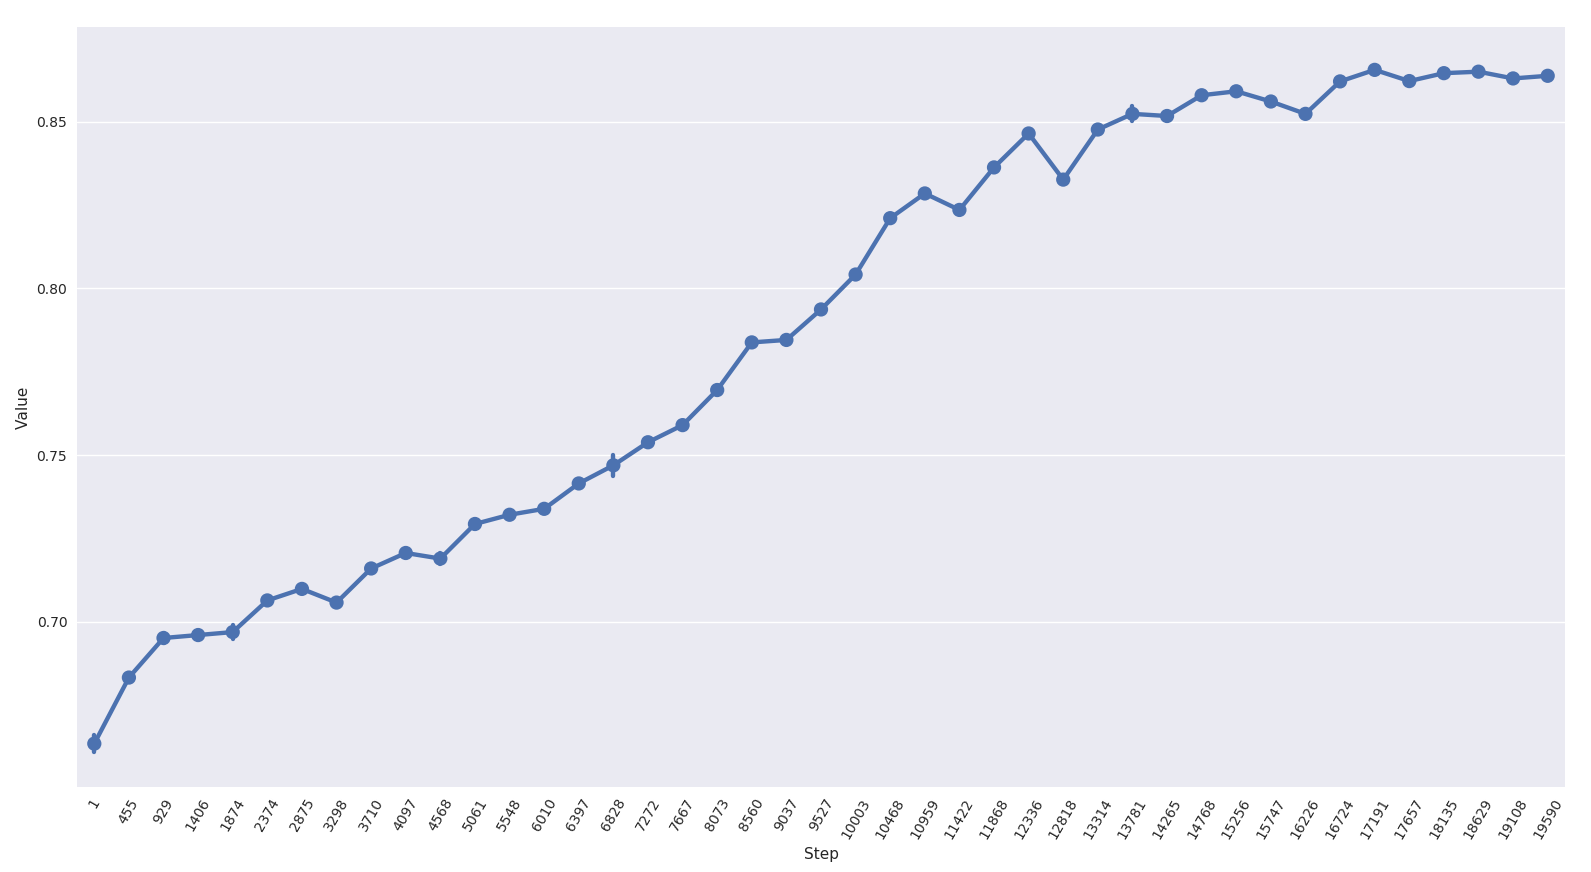
\includegraphics[width=.95\textwidth]{imgs/accuracy_wd_2}
  \caption{Evolución de la capacidad de predicción}
\end{figure}

Podemos ver en la gráfica que en los últimos 5000 pasos apenas se ha
conseguido mejorar el porcentaje de clasificación del modelo. No
obstante, con esta red hemos conseguido mejorar la capacidad de
aprendizaje de la misma, subiendo el porcentaje de acierto en
clasificación de un 73\% a un $86.5\%$. Esta mejora ha supuesto, si
tenemos en cuenta el error (27\% frente a $13.5\%$), conseguir
clasificar correctamente, en media, la mitad de los ejemplos que antes
no éramos capaces de clasificar. Supone por tanto una mejora muy
importante en el modelo. Además, hemos conseguido ganar mucha
estabilidad a la hora de la mejora del modelo, ya que como hemos
podido observar, la función de pérdida ha ido decrementando su valor
en todo momento, al contrario de lo que ocurría en el primer modelo,
en el que teníamos oscilaciones muy fuertes. Gran parte de la culpa de
este fenómeno es de los términos que hemos añadido, ya que el tener en
cuenta como penalización la norma de los pesos de la red, y
decrementarlos todos en cada paso de aprendizaje en función de su
norma, es normal que la función de pérdida no tienda a aumentar, ya que
la parte correspondiente a los pesos será mucho más significativa que
la correspondiente a la mala clasificación. No obstante, es innegable
que la implementación de \textit{Weight Decay} ha conseguido mejorar
enormemente los resultados obtenidos por la red, a la vista de los
resultados obtenidos.\\


\subsection{Segunda modificación: \textit{Variable Learning Rate} (vlr\_wd\_model)}

En vista de la mejora que nos supone el modelo anterior, trabajaremos
sobre éste y le añadiremos sucesivas modificaciones con fin de
estudiar la influencia de cada una en nuestro modelo. Hasta ahora
habíamos trabajado con una tasa de aprendizaje fija. Este parámetro
resulta difícil de ajustar, puesto que tenemos que encontrar un
equilibrio entre la capacidad de explorar el espacio de soluciones que
nos proporciona un valor de tasa de aprendizaje alto, y la capacidad
de optimizar los resultados en un entorno pequeño que conseguiríamos
con una valor bajo para la tasa.\\

Para solventar esta dificultad de ajustar el parámetro, y conseguir
una mayor flexibilidad entre la explotación y la exploración del
espacio de soluciones, utilizaremos una tasa de aprendizaje
variable. De esta forma se comienza con un valor de tasa de
aprendizaje relativamente alto, que nos permita realizar al inicio un
buen proceso de exploración, mientras este parámetro se reduce
gradualmente, dando así paulatinamente
más importancia al proceso de explotación.\\

Como ya se ha comentado, se utiliza la misma topología para nuestra
red neuronal que la que tenía el modelo anterior, utilizando también
el mismo esquema de aprendizaje con gradiente descendente, pero en
esta
ocasión con tasa de aprendizaje variable.\\

A continuación vamos a estudiar los resultados obtenidos en la
ejecución del nuevo modelo.

\subsubsection{Gráficas de resumen del aprendizaje}

De forma análoga a como se ha procedido hasta ahora, mostraremos las
gráficas sobre la función de pérdida y la capacidad de predicción del
modelo a lo largo de su fase de entrenamiento. En primer lugar
mostramos la función de pérdida:

\begin{figure}[H]
  \centering 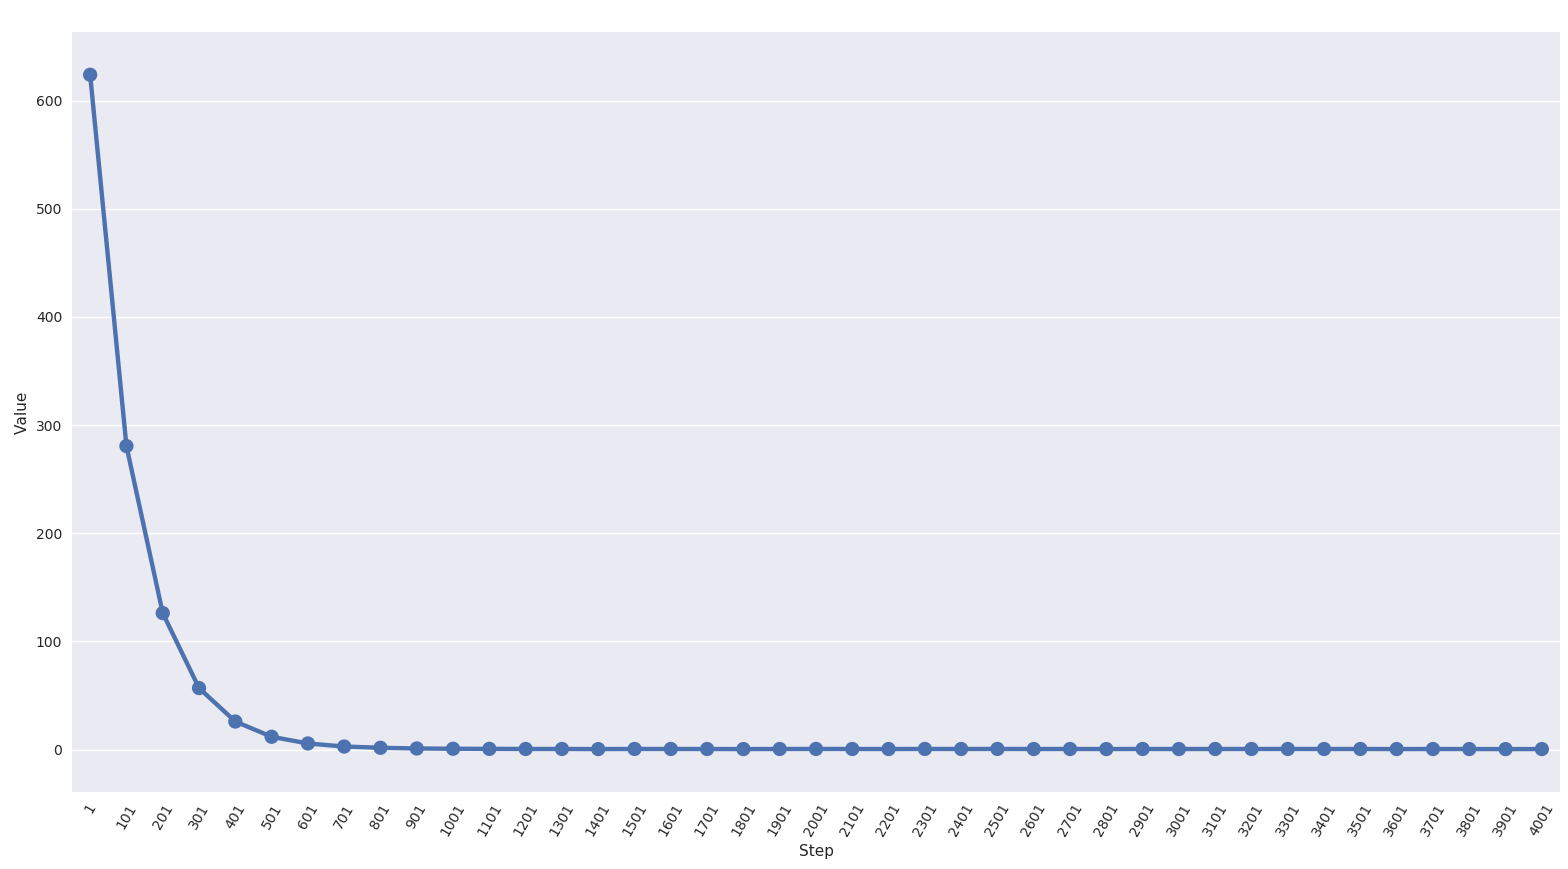
\includegraphics[width=.95\textwidth]{imgs/loss_vlr_wd}
  \caption{Evolución de la función de pérdida}
\end{figure}


Encontramos por un lado que la disminución de la función de pérdida es
mucho más rápida que la que obteníamos en el modelo anterior, bajando
muy rápidamente a valores inferiores a 10 y llegando por debajo de la
unidad, cuando el modelo anterior no era capaz obtener valores por
debajo de 100. Veamos a continuación como evoluciona la capacidad de
predicción del modelo actual.

\begin{figure}[H]
  \centering
  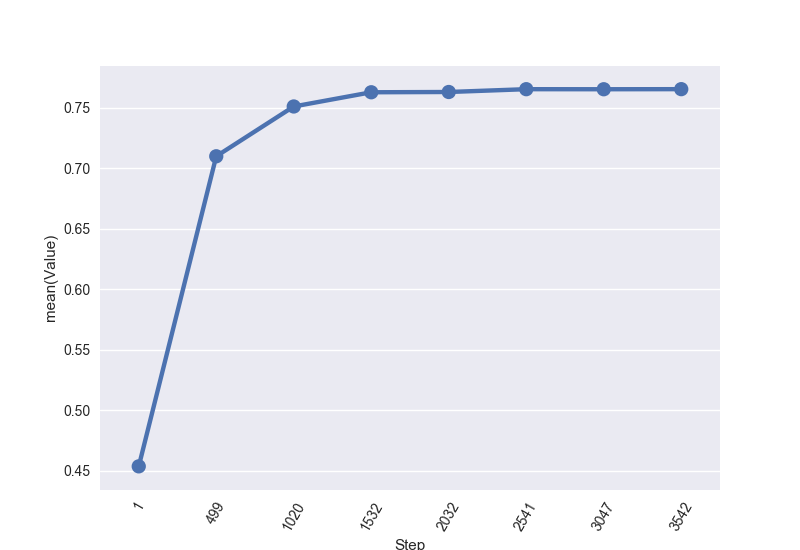
\includegraphics[width=.95\textwidth]{imgs/accuracy_vlr_wd}
  \caption{Evolución de la capacidad de predicción}
\end{figure}

En esta ocasión encontramos que aumenta muy rápidamente, pero pronto
se estanca, no consiguiendo alcanzar una precisión superior al
76\%. En vista de las dos gráficas anteriores, y del comportamiento
que obteníamos en el modelo anterior, podemos deducir que nuestro
modelo se centra demasiado en reducir el valor de pérdida provocado
por la penalización aplicada por el \textit{Weight Decay} en lugar de
mejorar la solución a nuestro problema.

\subsection{Tercera modificación: \textit{Variable Learning Rate} sin \textit{Weight Decay} (vlr\_model)}

Una vez estudiado el modelo anterior, nos cabe preguntarnos si el uso de
una tasa de aprendizaje variable nos puede ayudar en aquellos casos en los
que no apliquemos \textit{Weight Decay}, o lo apliquemos en una menor medida.\\

Con el fin de comprobar esta idea, creamos un nuevo modelo idéntico al 
anterior con la salvedad de que tan solo aplicaremos \textit{Weight Decay} en 
la capa densa. Nuestro propósito es comprobar que al no haber tanta 
penalización en la función de pérdida, nuestra red neuronal convolucional 
podrá realizar una mejor clasificación.\\

Pasámos a comprobar los resultados obtenidos por el tercer modelo:

\subsubsection{Gráficas de resumen del aprendizaje}

De nuevo pasamos a mostrar en primer lugar la evolución de la función
de pérdida, para a continuación estudiar la capacidad de predicción 
que nos aporta el modelo.

\begin{figure}[H]
  \centering 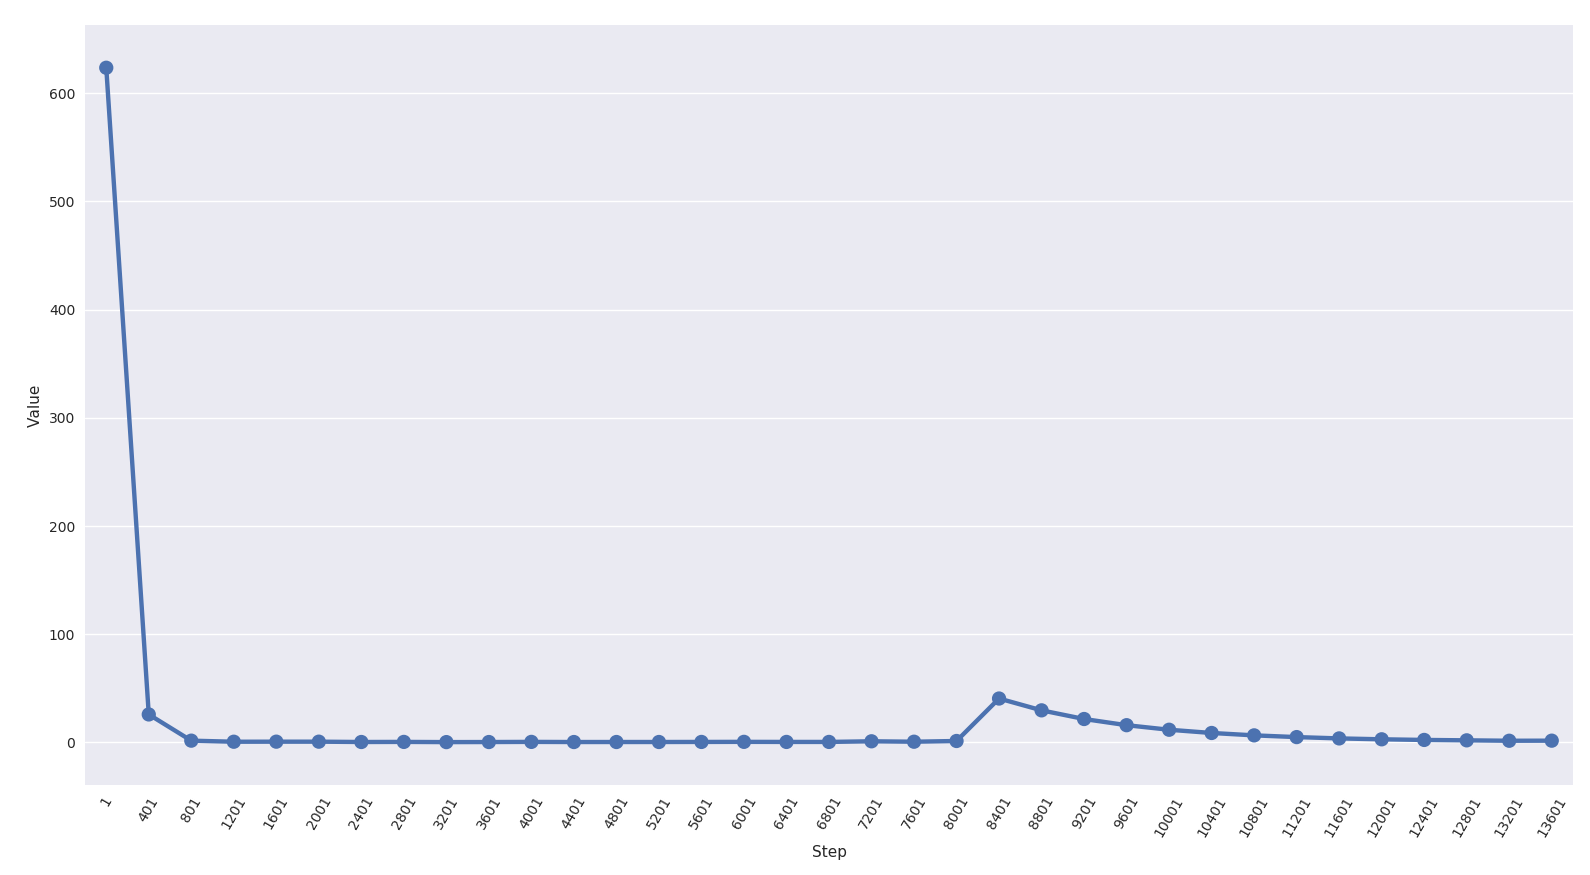
\includegraphics[width=.95\textwidth]{imgs/loss_vlr}
  \caption{Evolución de la función de pérdida}
\end{figure}


De nuevo encontramos que la función de pérdida, a pesar de comenzar con 
valores relativamente altos, rápidamente decrece y alcanza valores muy 
pequeños y se estabiliza. Sin embargo, encontramos que llega un punto 
en el que toma un alto valor. A pesar de que tras el salto vuelve a 
decrecer, lo hará de forma muy lenta y no llega a alcanzar los valores
en los que se situaba antes. Veamos cómo se comporta en la predicción:

\begin{figure}[H]
  \centering 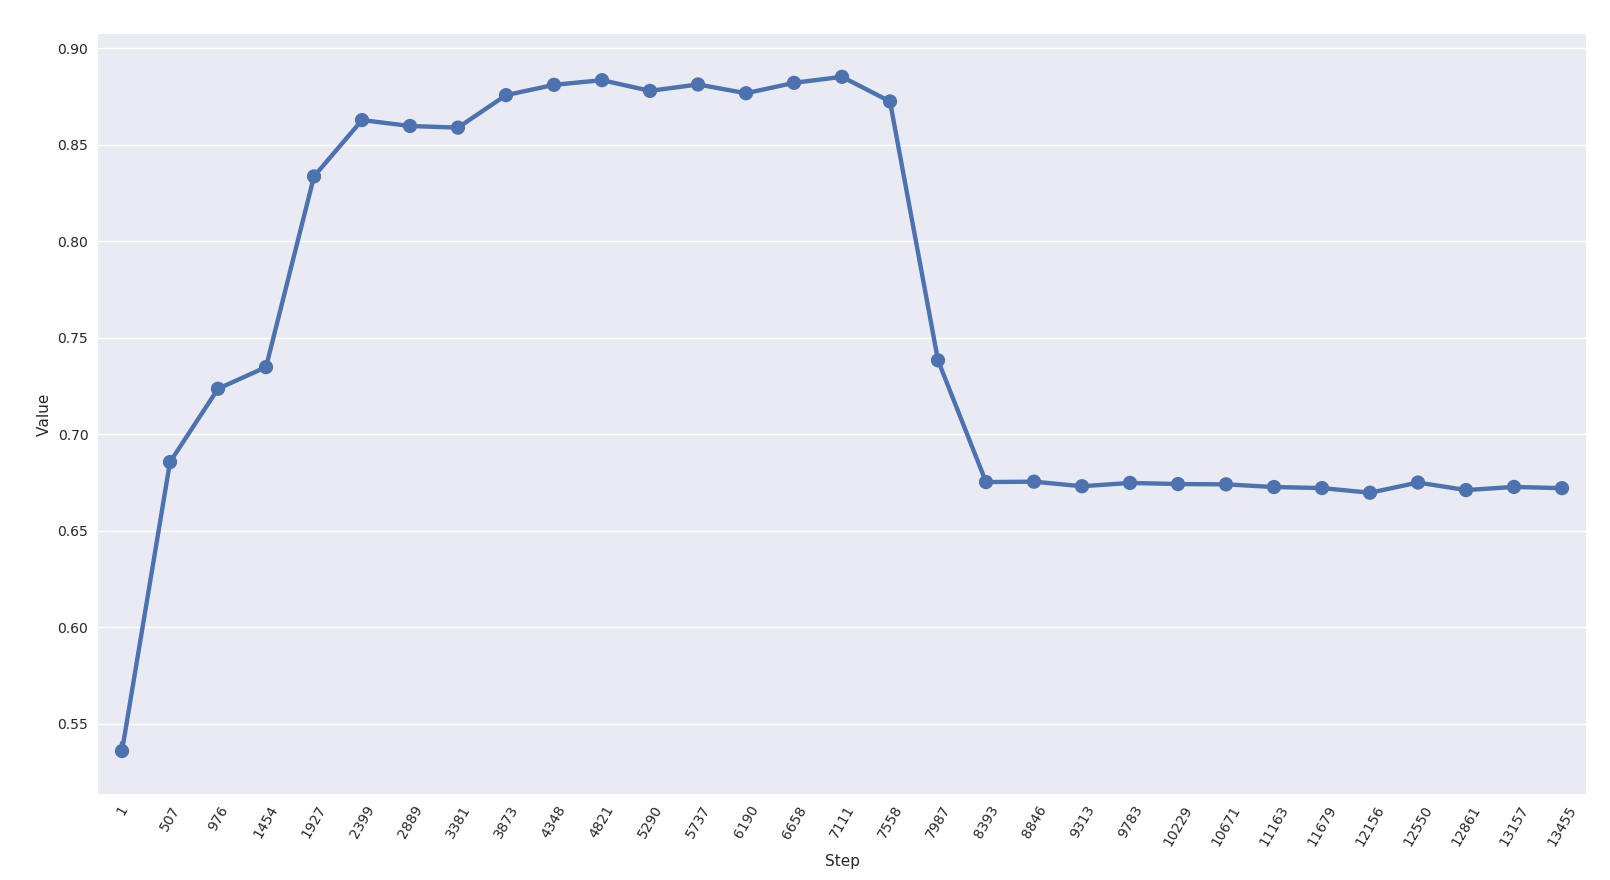
\includegraphics[width=.95\textwidth]{imgs/accuracy_vlr}
  \caption{Evolución de la capacidad de predicción}
\end{figure}

En esta ocasión encontramos, a diferencia del modelo anterior, que tras
una gran subida inicial, sigue creciendo, aunque de forma mucho más lenta.
A pesar de comenzar con una tasa de predicción por debajo del 55\%, este
modelo consigue alcanzar un 89\% de acierto, siendo notablemente mejor que
todo lo que habíamos conseguido hasta ahora.\\

Sin embargo, encontramos un rápido descenso coincidiendo con el punto en 
el que la función de pérdida aumentaba. La capacidad de predicción del 
modelo se reduce drásticamente estabilizándose en torno a un 66\%, valor 
muy inferior. Esto nos hace plantearnos que debemos establecer un criterio
de parada, para que la red neuronal finalice su entrenamiento y no se 
lleguen a estas situaciones.


\subsection{Sección de Paco}





\subsection{modificacion ADABOOST: esquema de aprendizaje mediante adamOptimizer (3adam\_model)}




\subsubsection{Gráficas de resumen del aprendizaje}



\printbibliography

\end{document}